\begin{figure}
\centering
\setlength{\figwidth}{0.5\columnwidth}
\resizebox{\columnwidth}{!}{
\begin{tabular}{c c}
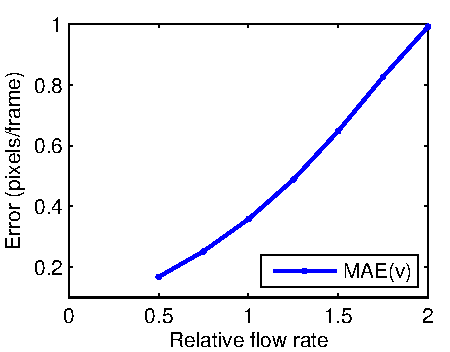
\includegraphics[width=\figwidth]{\figpath/flowrate} &
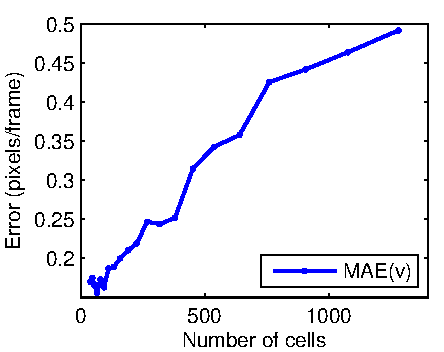
\includegraphics[width=\figwidth]{\figpath/n_cells} \\
(a) & (b) \\
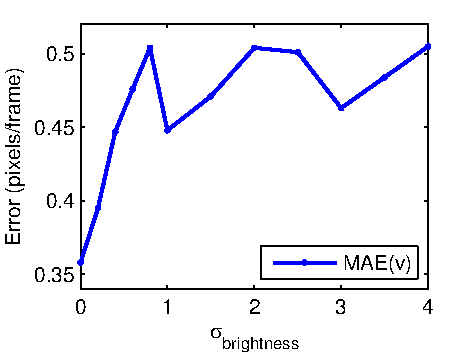
\includegraphics[width=\figwidth]{\figpath/brightness_sigma} &
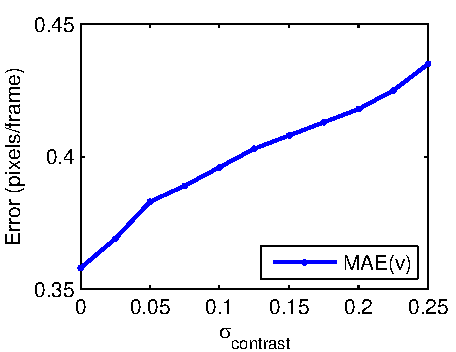
\includegraphics[width=\figwidth]{\figpath/contrast_sigma} \\
(c) & (d)
\end{tabular}}
%
\caption{Mean Absolute Error (MAE) in the vertical direction with respect to (a) relative flow rate, (b) number of simulated cells, (c) brightness variation and (d) contrast variation.}
\label{fig_flow_graphs_synth}
\end{figure}
